\chapter{Iterative Appliation Design (contributions)}
\label{contributions}

This chapter describes the contributions of all papers that are included in the thesis and them to the descriptions about application design as described in the previous chapter. The following sections first describe the separation of papers into topic areas and then elaborate on each of the topics.

\section{Overview}
\label{contributions:overview}
Due to the varied nature of application papers, this papers are separated into three topic areas:

\textbf{Biological and Medical Visualization. } \paperef{paperA} and \paperef{paperB} deal with algorithmic and application design challenges regarding biological simulation and medical intervention support respectively. \paperef{paperA} describes an algorithm that was developed to effieciently render non-linear finite element models; \paperef{paperB} describes an application system used in deep brain stimulation interventions.~(\SC{contributions:medbio})

\textbf{Urban Search \& Rescue. } \paperef{paperC}, \paperef{paperD}, and \paperef{paperE} describe the collaborative work on designing a visualization system to support urban search \& rescue operators and rescuers. The system utilizes \nD{3} point cloud data as the basis for a pathfinding algorithm, whose results are presented to the expert user for a human-in-the-loop decision support.~(\SC{contributions:usar})

\textbf{Astrophysical Phenomena. } The papers in this topic deal with visualization system that were performed to deal with astronomical and astrophysical phenomena. \paperef{paperF} and \paperef{paperH} describe visualization systems that are applied to space weather and ion simulations respectively, where as \paperef{paperG} describes the required algorithm necessary to achieve these systems.~(\SC{contributions:physics})

Each of the topics provides a short introduction into the domain and, then, elaborate on the work that has been done in the respective papers.

% For each contribution explain:
%   Problem domain
%   System that solves the problem
%   Collaboration with the experts
%   Evaluations
%   Generalizability (future work?)

\section{Biological and Medical Systems}
\label{contributions:medbio}
\begin{itemize}
\item Describe background and previous work in biological visualization + systems
\item Describe background and previous work in medical visualization + systems
\item Medical visualization as one of the first expert domains
\item Support for the operating theater
\item General problems with medical visualization
\begin{itemize}
    \item Hard to convince people to use it:
    \item Certification / limited time of the physicians
\end{itemize}
\end{itemize}

\subsection{Finite Element Visualization}
\label{contributions:medbio:fem}
\begin{itemize}
\item Other work: \cite{Liu12Fem}
\item Rendering multi-variate non-linear finite element models
\item Transformation from linear rays in world-space to curve rays in material space
\item Simulation values are described in material space
\item Transformation from world to material space is computationally expensive
\item Solve by using precomputation step to compute proxy rays for each element
\item Precomputation is allowable as the elements are usually not degenerate and smooth
\item During rendering time, proxy rays are used to look up values in the finite elements and perform the ray marching
\item Proxy ray computation
\begin{itemize}
    \item Create a uniform grid on the surfaces of each element
    \item Compute rays from each grid cell to each other grid cell
    \item Collect all proxy rays and store a limited number of control points used for Catmull-Rom spline interpolation 
    \item Move them into a common coordinate system (one point into origo, linear scaling, rotating all splines such that P0, Pp, Pn lie in the yz plane [P0 and Pn already on z axis from normalization], Pp is the first non-collinear point). Store $\theta$ from the rotation
    \item Perform clustering on the proxy rays \cite{abraham03clustering} with K-means \cite{hartigan75kmeans}
    \item Metric for clustering is the area covered between two splines
    \item Allow for potential different grid resolutions on entry v exit faces -> importance-based ray sampling
\end{itemize}
\item Rendering
\begin{itemize}
    \item Depth peeling \cite{mammen89DepthPeeling}
    \item Lookup ray id and $\theta$
    \item Bend and rotate closest ray into place
    \item Perform ray marching along the proxy ray (arc parametrization to take into account the different lenghts in material and world space \cite{guenter90arclength})
    \item Intersegment handling of sampling points (we do not want to start the sampling at the beginning, but have a continuous transition between elements)
    \item Inter vs intra ray interpolation
    \begin{itemize}
        \item Inter: bilinear lookup between four closest ray matches and perform interpolation between spline results
        \item Intra: Retrieving the opposite ray (entry->exit; exit->entry) and looking up at $t$ and $1-t$ and interpolate between
    \end{itemize}
\end{itemize}

\end{itemize}

\subsection{Deep Brain Stimulation Interventions}
\label{contributions:medbio:dbs}
\question{Is this too much a retelling of the paper story? If so, what additional information should be in here?}
In this work package, the task was to develop a medical visualization application for deep brain stimulation (DBS) intervention support in collaboration with physicians at the St.~Barbara Hospital in Hamm, Germany. Contrary to other medical domains, where the doctor's available preparation time for each patient is limited \todo{find citation for this} and thus procludes any complex interaction techniques on visualization applications, DBS interventions already have a long planning phase scheduled prior to the operation, thus enabling the usage of specialized tools.

The application that was developed combines an enhanced multimodal \nD{3} volume rendering environment with the spatial visualization of electric measurements that are recording during the procedure in combination with patient tests. Spatially embedding the measurements reduces the cognitive load of the surgeon. The system shows the varying uncertainties in a single view, thus enabling the surgeon more insight during the procedure.

\subsubsection{Background}
\label{contributions:medbio:dbs:background}
We investigated DBS interventions that were performed on patients' with Parkinson's Disease or other forms of tremors. During the interventions, a transmitting electrode is inserted into patients' brains that potentially inhibits some of the debilitating effects of these tremors~\cite{Lindberg2002}. A usual target region for the electrode is the patient's subthalamic nucleus~(STN), which has been shown to be a beneficial target~\cite{Benabid2009}. The problems with the STN is the relatively small size of a few millimeters~\cite{Richter2004}, the location deep inside the patient's brain, as well as the fact that in some patients it is not detectable in MRI scans~\cite{Starr2002} and thus hard to localize. Furthermore, a small deviation in the electrode's location will excite other parts of the patient's brain that can lead to memory or speech impairments.

In addition to traditional imaging modalities, the system makes use of Microelectrode Recordings~(MER)~\cite{Lenz1988} that record the electrical activities of the brain. The MER system consists of a small group of devices that measure the brain's electric field around them. The relative amplitude and frequency of these fields correlate with the brain region the electrode is in~\cite{benazzouz2002intraoperative} and can thus enable the surgeon to determine whether the electrodes are in the correct locations inside the patient's brain. The results of the MER recordings are traditionally reviewed on loudspeakers that are placed in the operating room. Aside from the obvious drawbacks of a limited auditory channel, potential background noise, and limited echoic memory, a big issue is the mental separation between the spatial location of the electrodes and their feedback. 

Problems that were not sufficiently solved by previous methods include the fusion of the available modalities. These modalities include pre-operative CT and MRI scans, interoperative X-Ray scans, the electrode measurements during the insertion, and patient tests after the final electrode has been activated. Making efficient use of all available information is important as the principal limiting factor for the maximum operation length is the patient's ability to cooperate, as a DBS intervention is very taxing to the patient as they have to be awake during the entire procedure which can last up to 10 hours.

A DBS procedure is split into three distinct phases. In the first phase, the \emph{planning} phase, the surgeon plans the operation by locating and segmenting the most probable location of the STN using preoperative CT and MRI scans. Using other tools, an optimal access channel is then planned that evades important brain regions. In the second phase, the \emph{recording} phase, the patient is in the operating room with their head in a stereotaxic frame, that restricts the movement and thus allows for a fixed-body transformation between the patient and the operating room, used for registration. The MER sensors are inserted into the patient's brain along the preplanned access path until they have reached the planned depth. If the electrodes correctly identify the STN region, the depth along the access path is noted and the electrodes are retracted. In the third phase, the \emph{placement} phase, a transmitting electrode is inserted into the access path to the depth that was measured during the previous phase. Once the electrode is in place, it is activated and its output is tuned. Using interoperative bi-planar X-ray scans and markers on the stereotactic frame, the location of the electrode inside the patient's brain is verified. Then, utilizing patient tests that examine the patients long term memory ability and measuring the tremor, the location of the electrode is fine tuned until an acceptable response is achieved or the patient is no longer capable of coorperating.

\subsubsection{System}
\label{contributions:medbio:dbs:system}
\question{Should I use ``I'' or ``we'' in the text?}
\begin{figure}
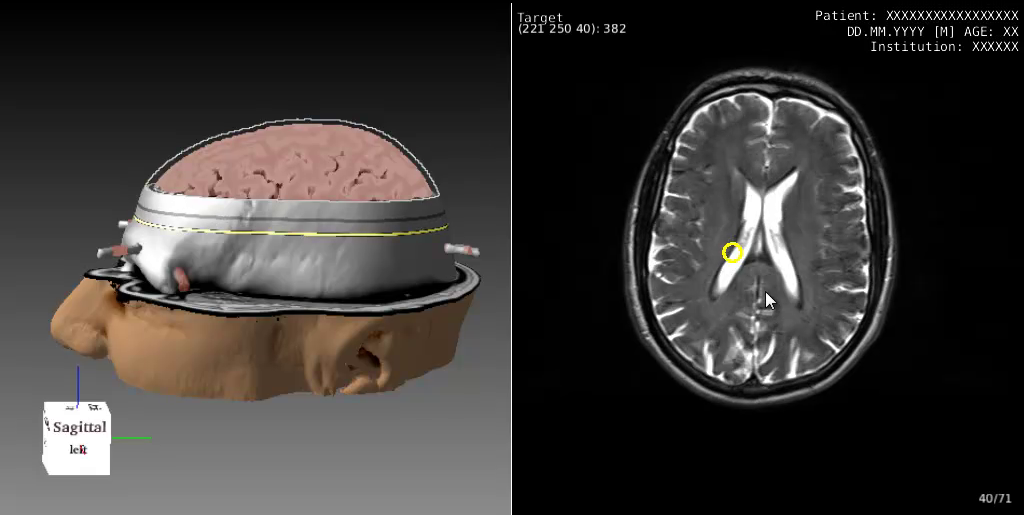
\includegraphics[width=\linewidth]{figures/contributions/dbs/planning.png}
\caption{This view shows the results of the use of a different planning tool to determine the entry point for the access path and the intented target location.}
\label{contributions:medbio:dbs:planning}
\end{figure}
We created a system that can ingest the access path planned using other sophisticated tools (see~\fref{contributions:medbio:dbs:planning}), the various scans, the MER measurements, and the patient tests during the operation. the system enables the surgeon to inspect all available information for each of the two operational phases. The \emph{Contextual view} is available in both phases, whereas the \emph{2D audio visualization} and \emph{3D audio visualization} are only available in the recording phase and the \emph{Target closeup} and \emph{Placement guide} are only available in the placement phase. The rest of this section elaborates on the design decisions for the individual views.

\question{How detailed should this be?}
\begin{figure}
\centering
\begin{subfigure}[b]{0.49\linewidth}
    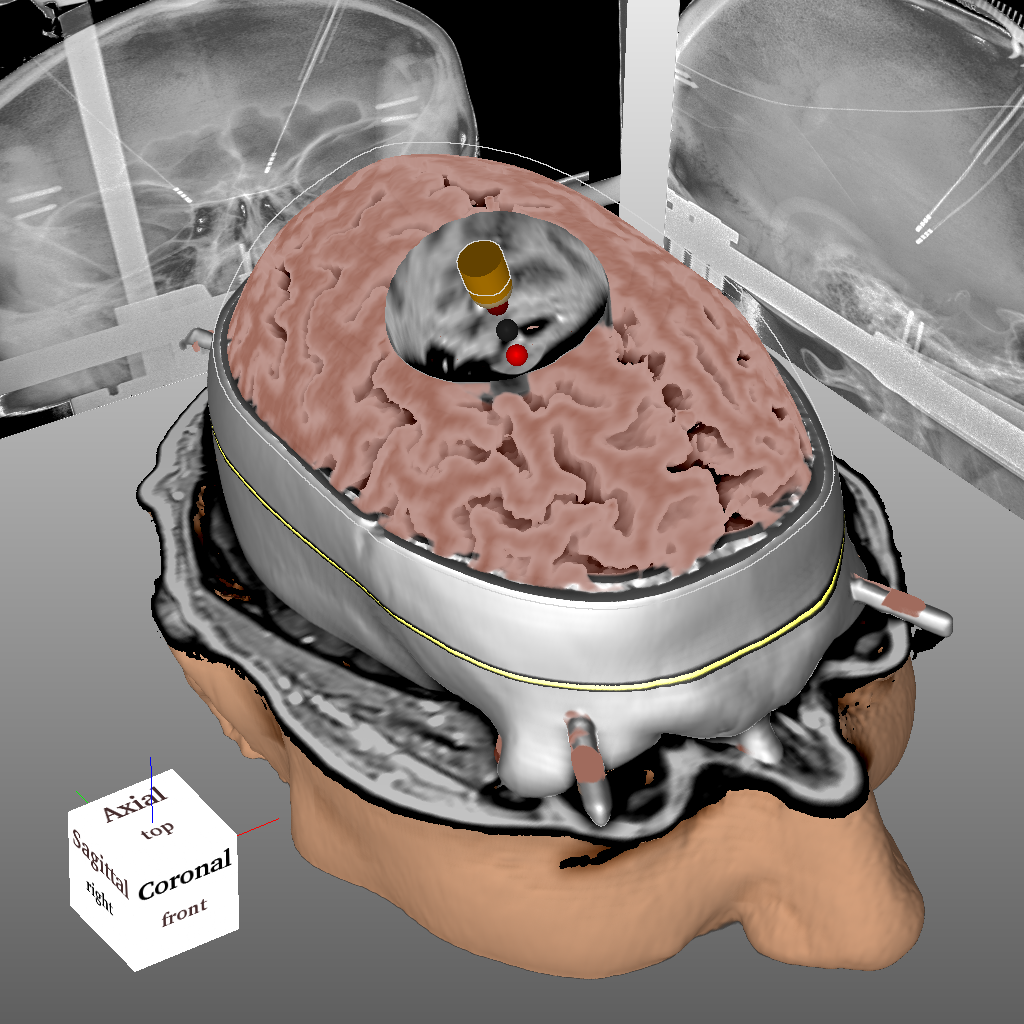
\includegraphics[width=\linewidth]{figures/contributions/dbs/recording-3d-1.png}
\end{subfigure}
\hfill
\begin{subfigure}[b]{0.49\linewidth}
    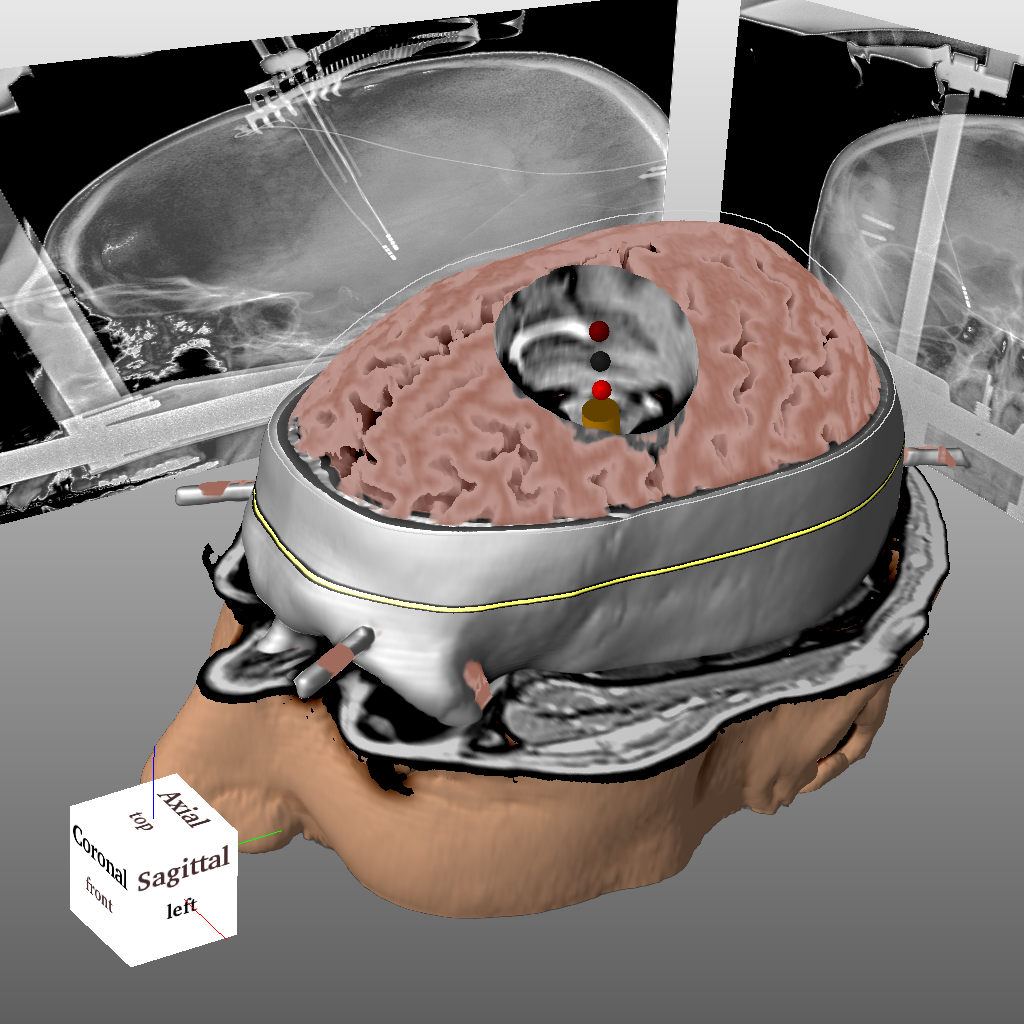
\includegraphics[width=\linewidth]{figures/contributions/dbs/recording-3d-2.png}
\end{subfigure}
% \includegraphics[width=\linewidth]{figures/contributions/dbs/recording-3d.png}
\caption{Presenting the \emph{Contextual View} that shows the multimodal fusion of all available datasets. The preoperative CT and MRI as well as the interoperative bi-planar X-ray scans are visible together with the animated location of the electrode. The colored beads along the access path show an automatic classification of the electrode measurements.}
\label{contributions:medbio:dbs:contextual}
\end{figure}

\paragraph{Contextual View} This \nD{3} view combines the preoperational CT and MRI scans together with the bi-planar X-rays, and the current electrode location (see~\fref{contributions:medbio:dbs:contextual}). The selected access path is presented in this view as a carved out tunnel. Explicitly showing the access path serves two purposes, first, it reduces the chance of a dangerous left-right mismatch error that might otherwise occur. Second, it enables us to place colored beads inside the access path behind the electrode. The colors of these beads depend on an automatic classification of the incoming electrode signal. This method was adopted from related works~\cite{Haese2005, Miocinovic2007}.

\paragraph{2D audio visualization} This view shows an augmented visualiation similar to an oscilloscope that presents the measurements from the available electrodes. As only the amplitude and frequency are important, we emphasize measurements that exceed a user-definable threshold and deemphasize the values below the threshold (see~\fref{contributions:medbio:dbs:sound:2d}). Furthermore, this view is linked with the \emph{3D audio visualization}, described below, such that when a specific electrode is selected in either view, it is highlighted in both views with a different color. This is used by the surgeon to be able to correlate the detailed measurements with the relative location of the electrode.
\begin{figure}
\centering
    \begin{subfigure}[b]{0.49\linewidth}
        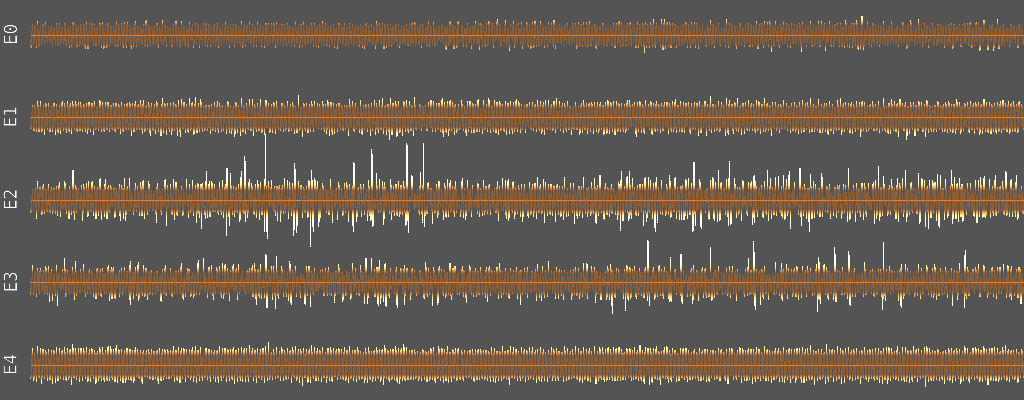
\includegraphics[width=\linewidth]{figures/contributions/dbs/audio-signal.png}
        \caption{The \nD{2} oscilloscope rendering of the electrode measurements presenting the accurate values.}
        \label{contributions:medbio:dbs:sound:2d}
    \end{subfigure}
    \hfill
    \begin{subfigure}[b]{0.49\linewidth}
        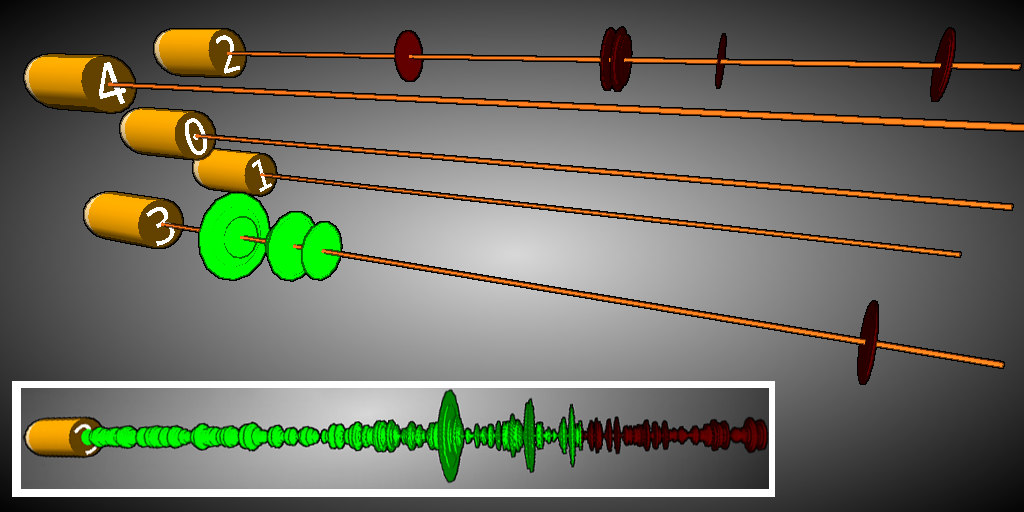
\includegraphics[width=\linewidth]{figures/contributions/dbs/recording-3dsound.png}
        \caption{The spatial \nD{3} rendering of the electrode rendering, showing their spatial location and rendering the high-amplitude measurements of the signal as colored discs.}
        \label{contributions:medbio:dbs:sound:3d}
    \end{subfigure}
    \caption{This figure shows the two rendering methods for displaying the measurements recorded by the Microelectrode Recording sensors. Both a view containing the accurate values are available (a) as well as a view showing the spatial relation between the electrodes.}
    \label{contributions:medbio:dbs:sound}
\end{figure}

\paragraph{3D audio visualization} In this separate view, the relative locations of the different electrodes are displayed (see~\fref{contributions:medbio:dbs:sound:3d}). The camera orientation is linked between this and the \emph{Contextual View} such that the mental registration between the two views is not broken. In this view, each electrodes' measurements that exceed a user-defined threshold are shown as discs that start at the electrode and move away from the electrode with increasing time. The size of the disc corresponds to the amplitude of the detected signal and thus shows the strength of the measured signal. The color of each disc is determined by the same classification algorithm that is used on the beads in the \emph{Contextual View}, but is simplified to show red if the electrode is outside of the STN and green if it is inside the STN. The surgeon can then, by correlating the frequency of discs and their amplitude verify that the classification was correct and that the electrodes are in the correct location.

\begin{figure}
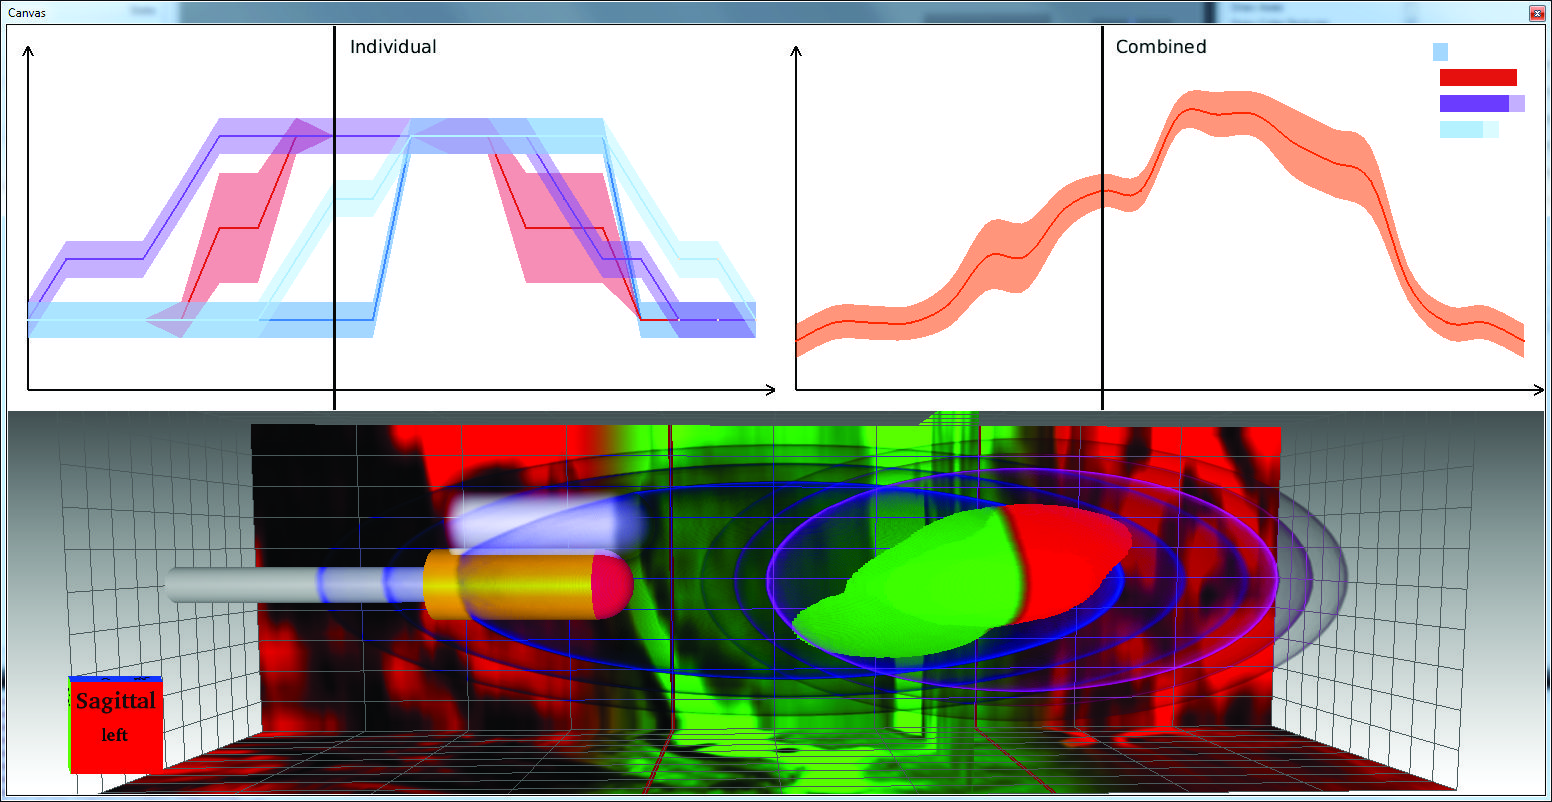
\includegraphics[width=\linewidth]{figures/contributions/dbs/screenshot-target.jpg}
\caption{The views that show the results of the different measurements performed during the recording phase. The \emph{Target closeup} (bottom view) contains the segmented location of the STN is visible as well as the results of the different tests at their spatial location. The \emph{Placement guide} shows the likelihood measurements according to their depth long the access path}
\label{contributions:medbio:dbs:target}
\end{figure}

\paragraph{Target closeup} After the potential electrode location has been determined, the surgeon uses this closeup view, centered around the segmented location of the STN, which combines all of the information that was gathered in the recording phase (see~\fref{contributions:medbio:dbs:target} bottom). Embedded in this view are the locations of the electrode as determined by the depth along the access path and as reconstructed by the biplanar X-ray scans. In addition it shows the MER signal results as a red-green overlay on the backside and presents options to add the patient test results as additional oval overlays. As all of these values have their own, unknown, uncertainty this view displays the overlap of the regions to inform the surgeon of the final placement that agrees with most measurements. On demand, the surgeon can enable the rendering of the MRI scan around the STN.

\paragraph{Placement guide} This view is based on the same information as the \emph{Target closeup}, but presents the information in a line plot, whose ordinate shows the likely hood of a correct placement for each measurement and the abcissa shows the depth along the access path (see~\fref{contributions:medbio:dbs:target} top). We display the uncertainty of each value by extruding the line with a transparent band.

\subsubsection{Evaluation}
\label{contributions:medbio:dbs:evaluation}

\subsubsection{Generalizability}
\label{contributions:medbio:dbs:generalizability}


\begin{itemize}
\item Good aspect about DBS operations: A long planning phase for the operation is already scheduled; less impact on using an extra tool
\item Deep Brain Stimulation operations  \cite{Benabid2009} \cite{Lindberg2002}
\item Subthalamic nucleus Size: \cite{Richter2004} Sometimes not detectable: \cite{Starr2002}
\item Parkinson's Disease
\item Previous systems
\item Microelectrode Recordings \cite{Lenz1988}
\item Multimodal fusion (CT, MRI, electrode measurements, X-Ray, Patient tests)
\begin{itemize}
    \item preoperative CT + MRI
    \item interoperative bi-planar X-Ray aligned to the electrode (patients head is inserted in a stereotaxic frame that ensures a fixed-body transformation between patient and operating room)
    \item MER electrode rendering
\end{itemize}
\item Desonification by showing the results instead of placing them on a loudspeaker
\item Removing the mental registration between electrode location and electrode measurements
\item three-step process
\begin{itemize}
    \item Planning phase outside the scope of the paper -> We implemented a tool to import desired path trajectory \cite{Shamir2010}
    \item Recording phase: Initial guiding to the correct location showing the MER measurements
    \item Placement phase: Presenting uncertainty from all measurements around the optimal placement location. Showing areas where the uncertain areas overlap -> Most likely the correct location
\end{itemize}
\item Limiting factor of the operation is the patient's ability to coorperate due to the long operating times (6-10 hours)
\item Working with the domain experts
\item Receiving their feedback and from them the data
\item System components
\begin{itemize}
    \item Contextual Component
    \begin{itemize}
        \item A \nD{3} view that fuses all available modalities. Shows MR scans (with vertical separation), bi-planar XRays, electrode location,
        \item Contextualization is an important aspect as left-right mismatches are a dangerous source of surgery error
        \item Presenting the location (= depth) of the electrode
        \item Recording measurements along the removed path (drawing \emph{beads} in the trajectory (shown in \cite{Haese2005} \cite{Miocinovic2007})). The color of each bead is determined by the MER classification.
        \item Showing the normalized location of the electrode on the bottom of the view. Combining the general spatial information of the main view with a detailed distance-based information of the inset
    \end{itemize}
    \item 2D audio visualization
    \begin{itemize}
        \item emphasize the important areas of the oscillogram (spikes)
        \item deemphasize the rest
        \item brushing and linking between this and the 3D audio visualization
    \end{itemize}
    \item 3D audio visualization
    \begin{itemize}
        \item separate view (orientation of the electrodes linked with the main view)
        \item Integrating MER data with the spatial information
        \item Rendering each electrode, which will drag disc behind it if the measurements were above a threshold. Colors correspond to the beads
        \item Disc size corresponds to the potential difference that was measured at that electrode
        \item Perspective distortion is not that important as the frequency is more important than the amplitude
    \end{itemize}
    \item Target closeup
    \begin{itemize}
        \item Shows the overlapping uncertainties for the differnet modalities as ellipses. Ellipses are approximations
        \item Shows X-ray determined location and distance determined location
        \item MER signal determination as red-green color overlay
        \item Optional overlay of MRI scan for this block
        \item Geometric model of the pre-segmented target location colored by where the most overlap between uncertainty regions is
    \end{itemize}
    \item Placement guide
    \begin{itemize}
        \item Showing same information as in the Target closeup, but as composable line plots
        \item Extruded lines to show uncertainty
    \end{itemize}
\end{itemize}
\item Evaluation
\begin{itemize}
    \item 5 neurosurgeons
    \item showcase video with following questionnaire

\end{itemize}
\item Generalizability
\begin{itemize}
    \item 3D audio visualization applicable for other data where spatial audio is recorded
    \item Target closeup view for overlapping uncertainty ranges
\end{itemize}
\end{itemize}

\section{Urban Search \& Rescue}
\label{contributions:usar}

\section{Astrophysics}
\label{contributions:physics}

\subsection{Space Weather Visualization}
\label{contributions:physics:spaceweather}
\cite{Bock14CME}

\subsection{Ion Beam Simulations}
\label{contributions:physics:ion}

\subsection{OpenSpace}
\label{contributions:physics:openspace}
\cite{Bock15bOpenSpace}
\cite{Bock15OpenSpace}

Adding CG\&A in submission?